\documentclass[a4paper, 12pt]{article}
% math symbols
\usepackage{amssymb}
\usepackage{amsmath}
\usepackage{mathrsfs}
\usepackage{physsummer}


\usepackage{enumitem}
\usepackage[margin = 2cm]{geometry}

\tolerance = 1000
\emergencystretch = 0.74cm



\pagestyle{empty}
\parindent = 0mm

\begin{document}

\setphysstyle{ГЦФО 8}{Серия Ш-09}{16.11.2016}

\setcounter{notask}{26}

\large

\taskpic{ Космонавт летит в капсуле и хочет попасть на корабль
  Гермес. Корабль и капсула двигаются перпендикулярно друг другу со
  скоростями $v=5$ м/с. В начальный момент расстояние от капсулы до
  точки пересечения её траектории и траектории корабля равно $3.2$ км,
  а корабль находится на расстоянии $1.8$ км до этой точки. В любой
  момент космонавт может катапультироваться и вылететь вбок
  относительно капсулы со скоростью $3$ м/с. Когда именно космонавту
  следует катапультироваться, чтобы попасть на корабль? }
{
  \begin{tikzpicture}
    \draw[thick, dashed] (0,0) -- (3,0);
    \draw[thick, dashed] (3,-3) -- (3,0);
    \draw[thick,fill=white] (3,-3) circle (0.2cm) node[left=0.3cm]
    {Капсула};
        \draw[thick,fill=white] (0,0) circle (0.2cm) node[below=0.3cm]
    {Гермес}; 
    \draw[thick,->] (0.2,0) -- ++(0.8,0) node[above] {$v$};
    \draw[thick,->] (3,-2.8,0) -- ++(0,0.8) node[left] {$v$}; 
  \end{tikzpicture}
}
% СПб, район 2015-8

\taskpic[6cm]{ Метеорологический зонд состоит из лёгкого и жёсткого шара
  средней плотностью $\rho=0.3 \kgm$ и объёмом $V=5 \text{ м}^3$ и
  полезной аппаратуры малого объёма и массы $m=0.5$ кг. На какую
  высоту поднимется зонд? Зависимость плотности атмосферы $\rho_a$ от
  высоты известна и представлена на графике. Считать, что объём и
  плотность шара не зависят от внешних условий.  }
{
  \begin{tikzpicture}[/pgfplots/axis labels at tip/.style={ xlabel
      style={at={(current axis.right of origin)}, yshift=2 ex,
        xshift=3 ex,
        anchor=east,fill=white}, ylabel style={at={(current axis.above
          origin)}, yshift=1.3 ex, xshift=1 ex, anchor=north west,fill=white}}]
    \begin{axis}[
      width=6cm,
      xmin=0,xmax=14,ymin=0,ymax=1.3,
      axis x line=bottom,
      axis y line=middle,
      axis labels at tip,
      xlabel={$h$, км},
      ylabel={$\rho_a$, $\text{кг/м}^3$},
      minor xtick={1,3,5,...,13},
      minor ytick={0.1,0.3,...,1.1},
      xtick={0,2,4,...,12},
      ytick={0,0.2,0.4,...,1.2},
      tick label style={font=\small},
      label style={font=\small},
      grid=both]
      \addplot[domain=0:14,very thick,red,mark=none] {1.2*exp(-0.115*x)};
    \end{axis}
  \end{tikzpicture}
}
% СПб, район 2014-8

\taskpic[6cm]{ Экспериментатор собрал из подручных материалов робота. Робот
  потребляет фиксированную мощность $P_0=20$ Вт и тратит её на то,
  чтобы закручивать шурупы. Робот не идеален, и часть мощности
  расходуется впустую, нагревая самого робота. График КПД робота
  $\eta$ от его температуры приведён на рисунке. Какое количество
  шурупов закрутит робот за десять минут работы в установившемся
  температурном режиме? Для того, чтобы закрутить шуруп, необходимо
  совершить работу $A=40$ Дж. Мощность теплоотдачи в окружающую среду
  пропорциональна разности температур робота и среды и даётся
  выражением $\alpha (T - T_{\text{окр}})$, $\alpha = 0.6\text{
    Вт}/^{\circ}\text{C}$, $T_{\text{окр}} = 20^{\circ}\text{C}$.  }
{
  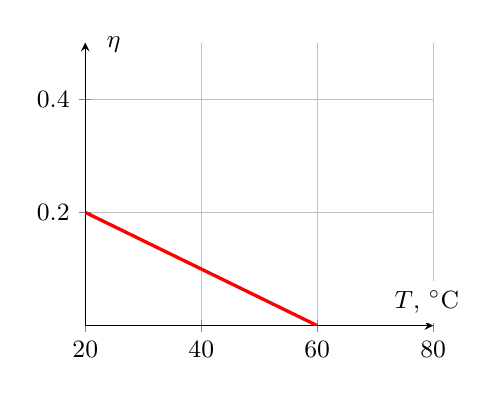
\begin{tikzpicture}[/pgfplots/axis labels at tip/.style={ xlabel
      style={at={(current axis.right of origin)}, yshift=2 ex,
        xshift=3 ex,
        anchor=east,fill=white}, ylabel style={at={(current axis.above
          origin)}, yshift=1.3 ex, xshift=1 ex, anchor=north west,fill=white}}]
    \begin{axis}[
      width=6cm,
      xmin=20,xmax=80,ymin=0,ymax=0.5,
      axis x line=bottom,
      axis y line=middle,
      axis labels at tip,
      xlabel={$T$, ${^{\circ}\text{C}}$},
      ylabel={$\eta$},
      % xtick={20,60},
      % ytick={0,0.2},
%      yticklabels={0,0.2},
      tick label style={font=\small},
      label style={font=\small},
      grid=both]
      \addplot[domain=0:80,very thick,red,mark=none] coordinates {(20,0.2) (60,0)};
    \end{axis}
  \end{tikzpicture}
}
% СПб, район 2015-8


\end{document}

%%% Local Variables: 
%%% mode: latex
%%% TeX-engine:xetex
%%% TeX-PDF-mode: t
%%% End:
